\scanpage{47}
\[
\det\bigl((c_{ij})_{1\leq i,j\leq n}\bigr)\overset{?}{=}
\qquad c_{ij}=0\quad\text{si }i\neq j,\ i,j\ \text{non consécutifs}
\]
\[
\sum_{\sigma\in\unsure{\mathfrak S}_n}
\varepsilon_\sigma\overset{\unsure{*}}{\prod_{i=1}^{n}}
\underbrace{c_{i\,\sigma(i)}}_{\text{nul, sauf si }\sigma\ \text{est tel que}}
\qquad
\overbrace{\forall i\in[1,n],\quad\sigma i\in\{i-1,i,i+1\}}^{\sigma\ \text{admissible}}
\]
Supposons $n\geq\unsure{2|3}$, alors tt cycle de $\sigma$ est de longueur $1$ ou $2$
et les cycles de long. $2$ \unsure{sont formés} d'indices consécutifs,
donc $\sigma$ est de la forme
\[
\sigma_{i_1}\sigma_{i_2}\mathbin{-}\sigma_{i_p}
\qquad1\leq i_1<i_2\mathbin{-}<i_p\leq n-1
\]
($\sigma_i$ est la transposition de $i,i+1$), où $i_1\ i_2\mathbin{-}i_p$
sont des entiers non consécutifs.
\margin{\figure{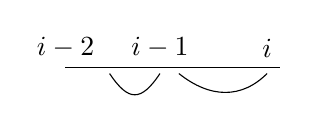
\begin{tikzpicture}[scale=.8]
\draw (0,0)--(3.4,0);
\node[above] at (0,0){$i-2$};\node[above] at (1.5,0){$i-1$};\node[above] at (3.2,0){$i$};
\draw (.7,-.1) .. controls (1,-.55) and (1.2,-.55) .. (1.5,-.1);
\draw (1.8,-.1) .. controls (2.3,-.5) and (2.8,-.5) .. (3.2,-.1);
\end{tikzpicture}}}
\[
\underbrace{1+\alpha_{\unsure{0|1}}}_{i_1}\quad
\underbrace{\deleted{\unsure{i_1+}}3+\alpha_{\unsure{0|1}}+\alpha_2}_{i_2}\quad
\underbrace{\unsure{i_1+}5+\alpha_{\unsure{0|1}}+\alpha_2+\alpha_3}_{i_3}
\mathbin{-}
\underbrace{\deleted{\unsure{i_1+}}(2\unsure{p}-1)+\alpha_{\unsure{0|1}}\mathbin{-}+\alpha_p}_{i_p}
\]
\deleted{$\displaystyle
\sum_{\substack{i_1\,i_2\,\mathbin{-}\,i_p\\
\text{\unsure{entiers} str. cr.}\\\text{distants}}}$}
\[
\deleted{1\leq i_1\qquad1+\alpha_1\mathbin{-}+\alpha_{p-1}\leq}
\]
\[
\alpha_i\in\mathbb N\qquad
\alpha_0\mathbin{-}+\alpha_{p-1}\leq n-2p
\]
\[
\begin{aligned}
&\sum_{1\leq p\leq[\frac n2]}(-1)^p
\sum_{\substack{(\alpha_{\unsure{0|1}},\ldots,\alpha_{\unsure{p-1|p}})\in\mathbb N^p\\
\sum\alpha_i=n-2p}}
\deleted{\unsure{\prod_i}}
\prod_{\substack{1\leq i\leq n\\
\text{non de la forme}\\
\left\{\begin{smallmatrix}(2r-1)+(\alpha_{\unsure{0|1}}\mathbin{-}+\alpha_r)\\
2r+(\alpha_{\unsure{0|1}}\mathbin{-}+\alpha_r)\end{smallmatrix}\right.\\
1\leq r\leq p}}
c_{ii}\\
&\hspace{3em}\prod_{1\leq r\leq p}
\left(
c_{2r-1+(\alpha_1+\cdots+\alpha_r),\,2r+(\alpha_1+\cdots+\alpha_r)}
c_{2r+(\alpha_1+\cdots+\alpha_r),\,2r-1+(\alpha_1\mathbin{-}+\alpha_r)}
\right)
\end{aligned}
\]
Supposons matrice \uline{symétrique}, et
$c_{i\,i+1}=-c_{i+1}\qquad c_{ii}=2c_i$.

On trouve
\[
\det\bigl((c_{ij})\bigr)_{1\leq i,j\leq n}
=\sum_{1\leq p\leq[\frac n2]}(-1)^p
2^{\inserted{\text{\figure{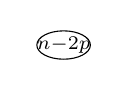
\begin{tikzpicture}[baseline=-.5ex]
\draw (0,0) ellipse (.34 and .18);\node at (0,0){$\scriptstyle n-2p$};
\end{tikzpicture}}}}}
\sum_{\substack{\alpha_*\in\mathbb N^p\\
\alpha_1\mathbin{-}+\alpha_p\leq n-2p}}
\prod_i c_i
\prod_{1\leq r\leq p}
(c_{2r+\alpha_1\mathbin{-}+\alpha_r})^2
\]
\figure{\begin{tikzpicture}[x=.65cm,y=.65cm]
\fill (0,0) circle (.035);\node[below] at (0,-.08){$c_1$};
\draw (.4,0)--(1.2,0);\draw (.4,-.08)--(.4,.08);\draw (1.2,-.08)--(1.2,.08);
\node[below] at (.65,-.08){$c_2$};
\draw (1.4,0)--(2.35,0);\draw (1.4,-.08)--(1.4,.08);\draw (2.35,-.08)--(2.35,.08);
\node[below] at (1.4,-.08){$c_3$};
\fill (2.5,0) circle (.055);\draw (2.5,0)--(3.2,0);\fill (3,0) circle (.07);
\draw (3.3,-.08)--(3.3,.08);\draw (3.3,0)--(4.2,0);\draw (4.2,-.08)--(4.2,.08);
\fill (4.5,0) circle (.035);
\draw (4.8,-.08)--(4.8,.08);\draw (4.8,0)--(6,0);\draw (6,-.08)--(6,.08);
\node at (6.65,0){$\cdots$};
\draw (7.3,-.08)--(7.3,.08);\draw (7.3,0)--(8.8,0);\fill (8.8,0) circle (.035);
\node at (9.4,0){$\cdots$};\node[below] at (9.8,-.08){$c_n$};
\fill (-.4,-.65) circle (.025);\node at (-2,-1.65){$c$};
\end{tikzpicture}}
\mspage{46}

